\documentclass[14pt,aspectratio=169,hyperref={pdftex,unicode},xcolor=dvipsnames]{beamer}
\usepackage[english,russian]{babel}
\usepackage[utf8x]{inputenc}
\usepackage[T2A]{fontenc}
\usepackage{cmap}
\usepackage{paratype}
\usepackage{hyperref}
\usepackage{qrcode}

\usetheme{metropolis}
\usefonttheme[]{professionalfonts}  % запрещаем beamer'у перезаписывать мат. шрифты
\metroset{numbering=fraction}
\metroset{subsectionpage=progressbar}

\setbeamercolor{frametitle}{fg=black}
\setbeamertemplate{frametitle}
{
 \vspace{3mm}\insertframetitle\par
}
\setbeamertemplate{title separator}{}
\setbeamertemplate{footnote separator}{}


\usebackgroundtemplate{
\includegraphics[width=\paperwidth,height=\paperheight]{./common/background_white.jpg}}

\logo{\vspace{-1.2cm}
\includegraphics[width=6mm]{./common/short-v.pdf}\hspace*{1.08\textwidth}}

\institute
{
  \begin{columns}
    \begin{column}{1.5cm}
    
\includegraphics[height=15mm,keepaspectratio]{./common/math-cs.pdf}
    \end{column}
    \begin{column}{4cm}
          Факультет математики и компьютерных наук СПбГУ
    \end{column}
  \end{columns}
}


\begin{document}

\begin{frame}[plain]
  \begin{center}
    \textbf{Никита Митцев}

    {\Large\textbf{Разработка ограничителя частоты запросов для Яндекс.Трекера}}


    {\small Руководитель проекта: Эдуард Александров}

    23.12.2002
  \end{center}


  \begin{columns}
    \begin{column}{1cm}
    
\includegraphics[height=15mm,keepaspectratio]{./common/math-cs.pdf}
    \end{column}
    \begin{column}{10cm}
      \small
          Факультет математики и~компьютерных наук СПбГУ\\
          Программа <<Современное программирование>>
    \end{column}
  \end{columns}
\end{frame}


\begin{frame}
\frametitle{Что такое Трекер}
\begin{center}
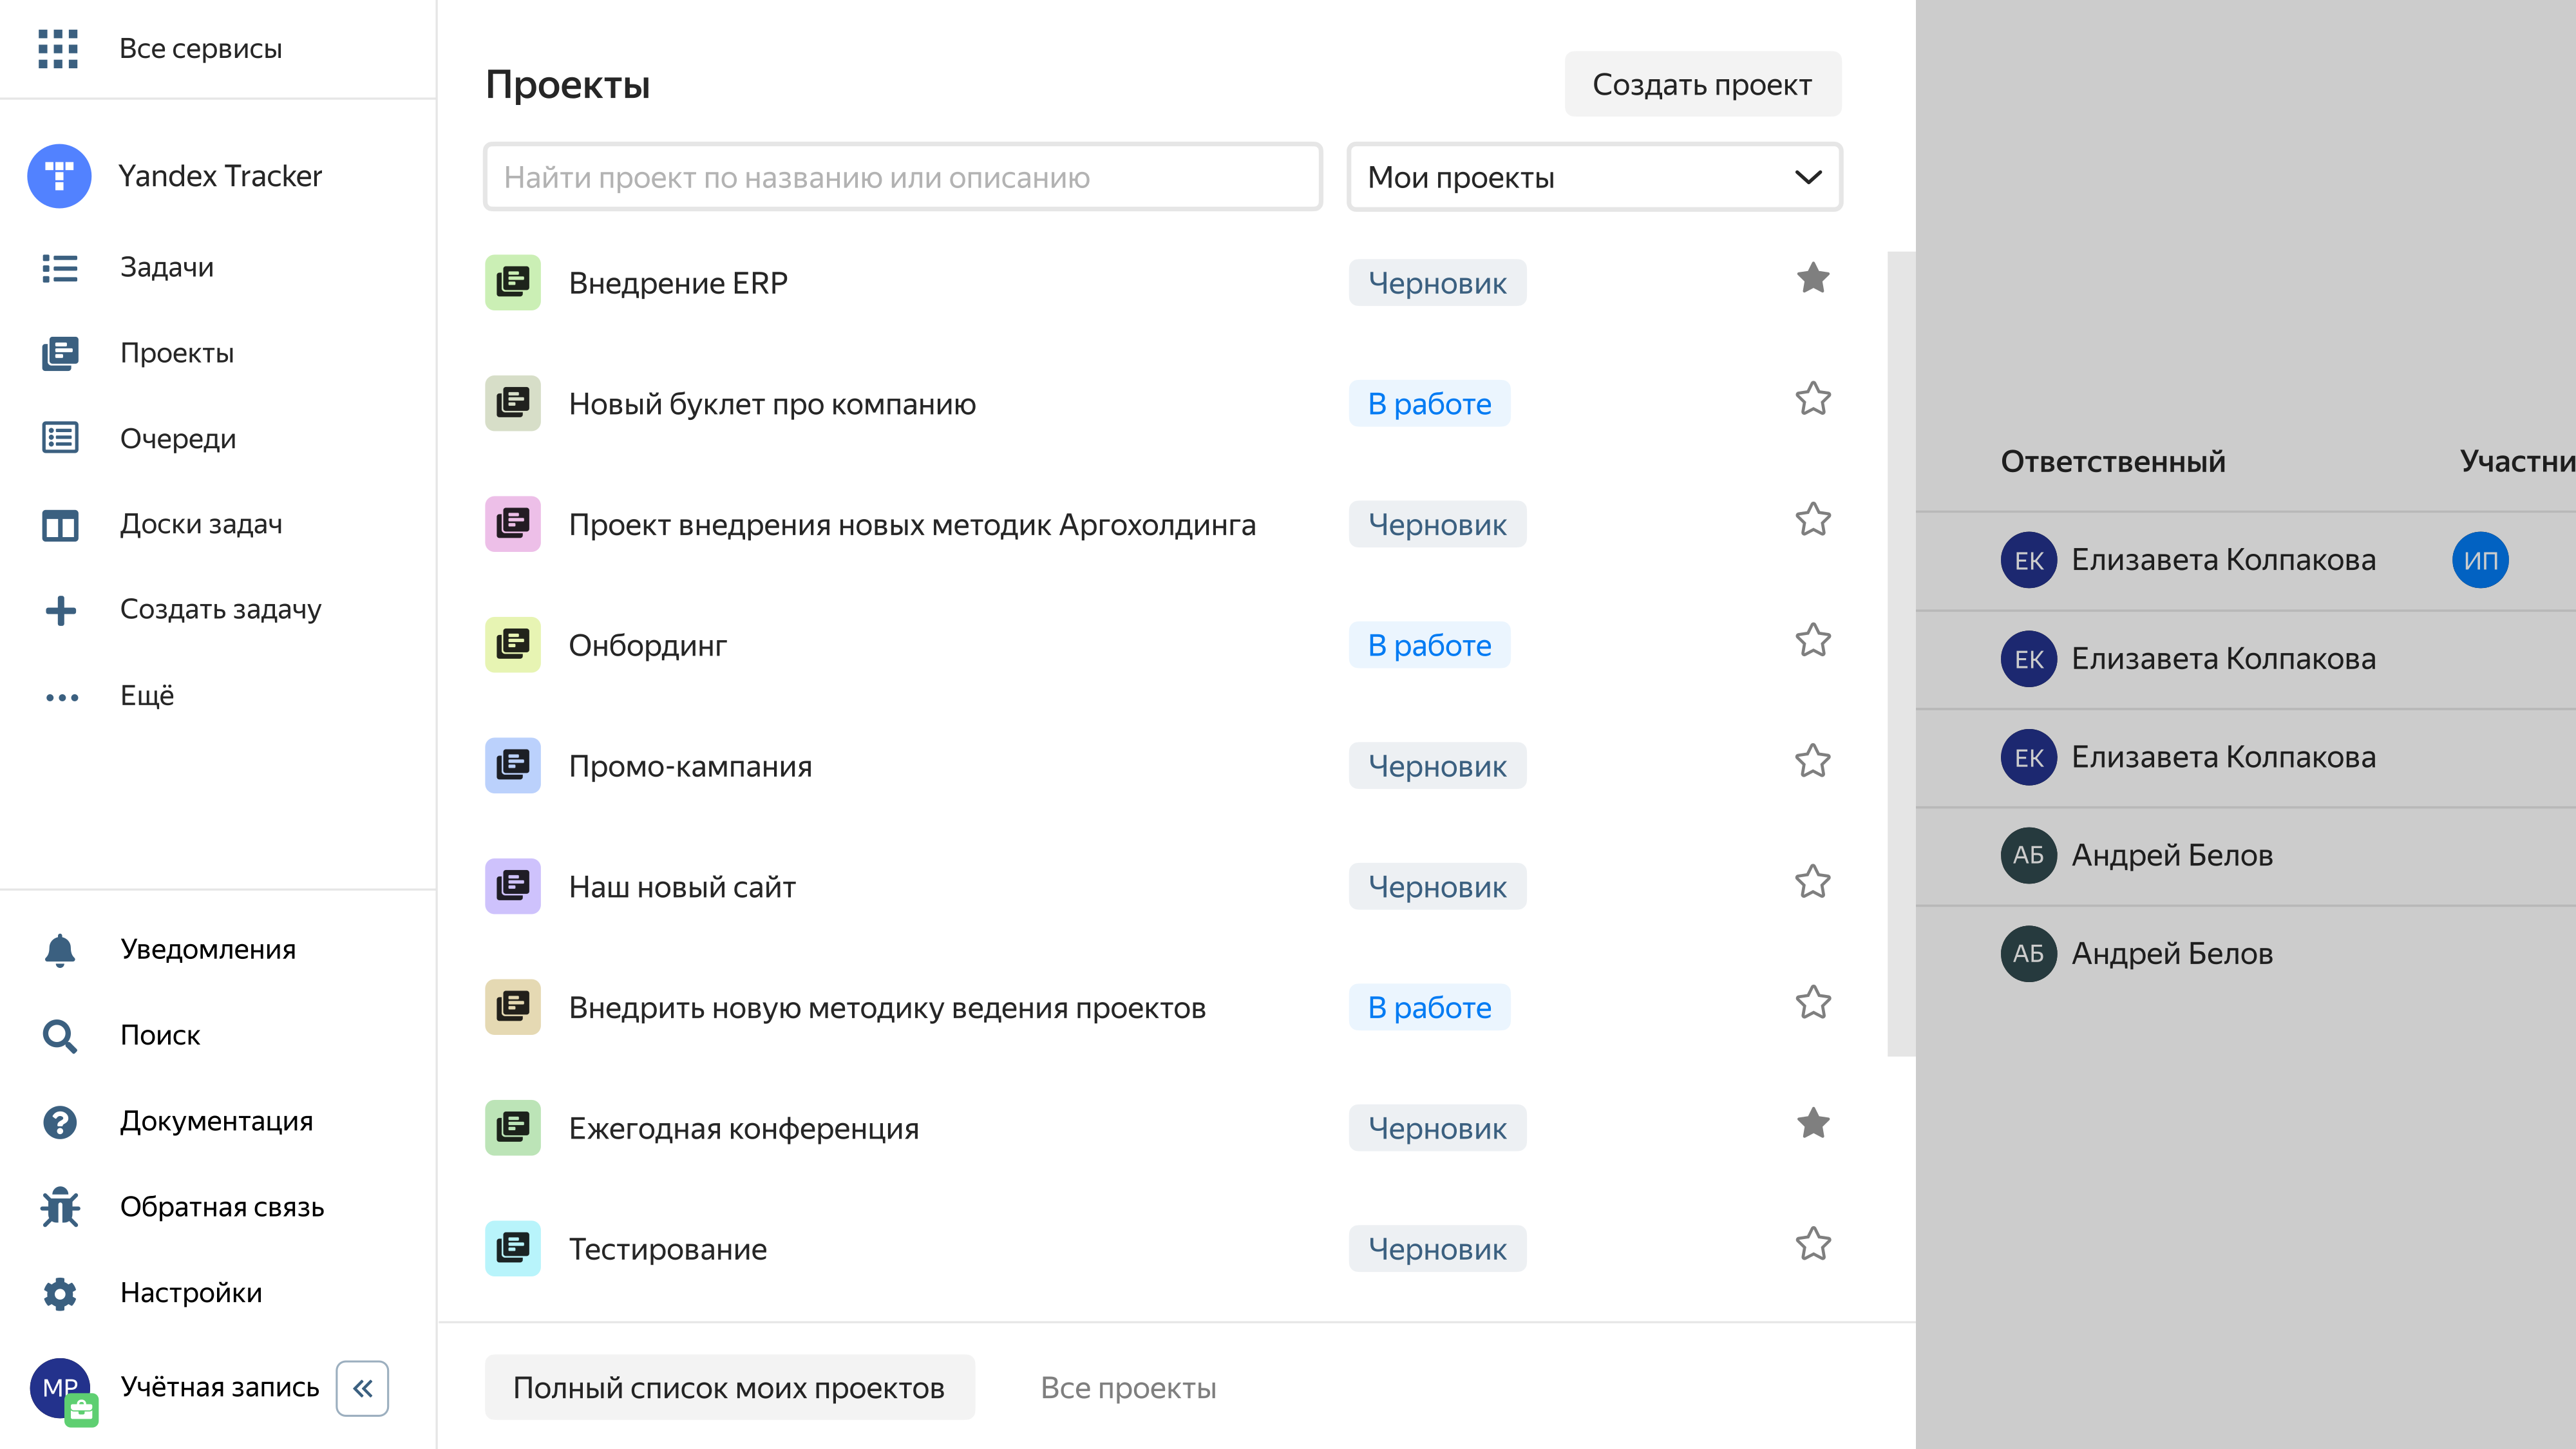
\includegraphics[width=12cm]{images/tracker.png}
\end{center}
\end{frame}

\begin{frame}
\frametitle{Зачем Трекеру ограничивать запросы}

\begin{itemize}
\item Обращение к некоторым подсистемам вычислительно намного дороже, чем к остальным. Их перегрузка может нарушить работу сервера.
\item Пользователи иногда пишут ужасные скрипты, обращающиеся к ним по 500 раз.
\item Этой же уязвимостью могут воспользоваться злоумышленники
\end{itemize}

\end{frame}

\begin{frame}
\frametitle{Задачи}
\begin{enumerate}
\item Установить проблемы и требования.
\item Исследовать существующие решения.
\item Согласовать и реализовать подход.
\item Протестировать корректность и производительность.
\end{enumerate}
\end{frame}

\begin{frame}
\frametitle{Последовательность обработки запроса}
\begin{center}
\includegraphics[width=14cm]{images/interceptor.png}
\end{center}
\end{frame}


\begin{frame}
\frametitle{Распределенная структура бэкенда}
\begin{center}
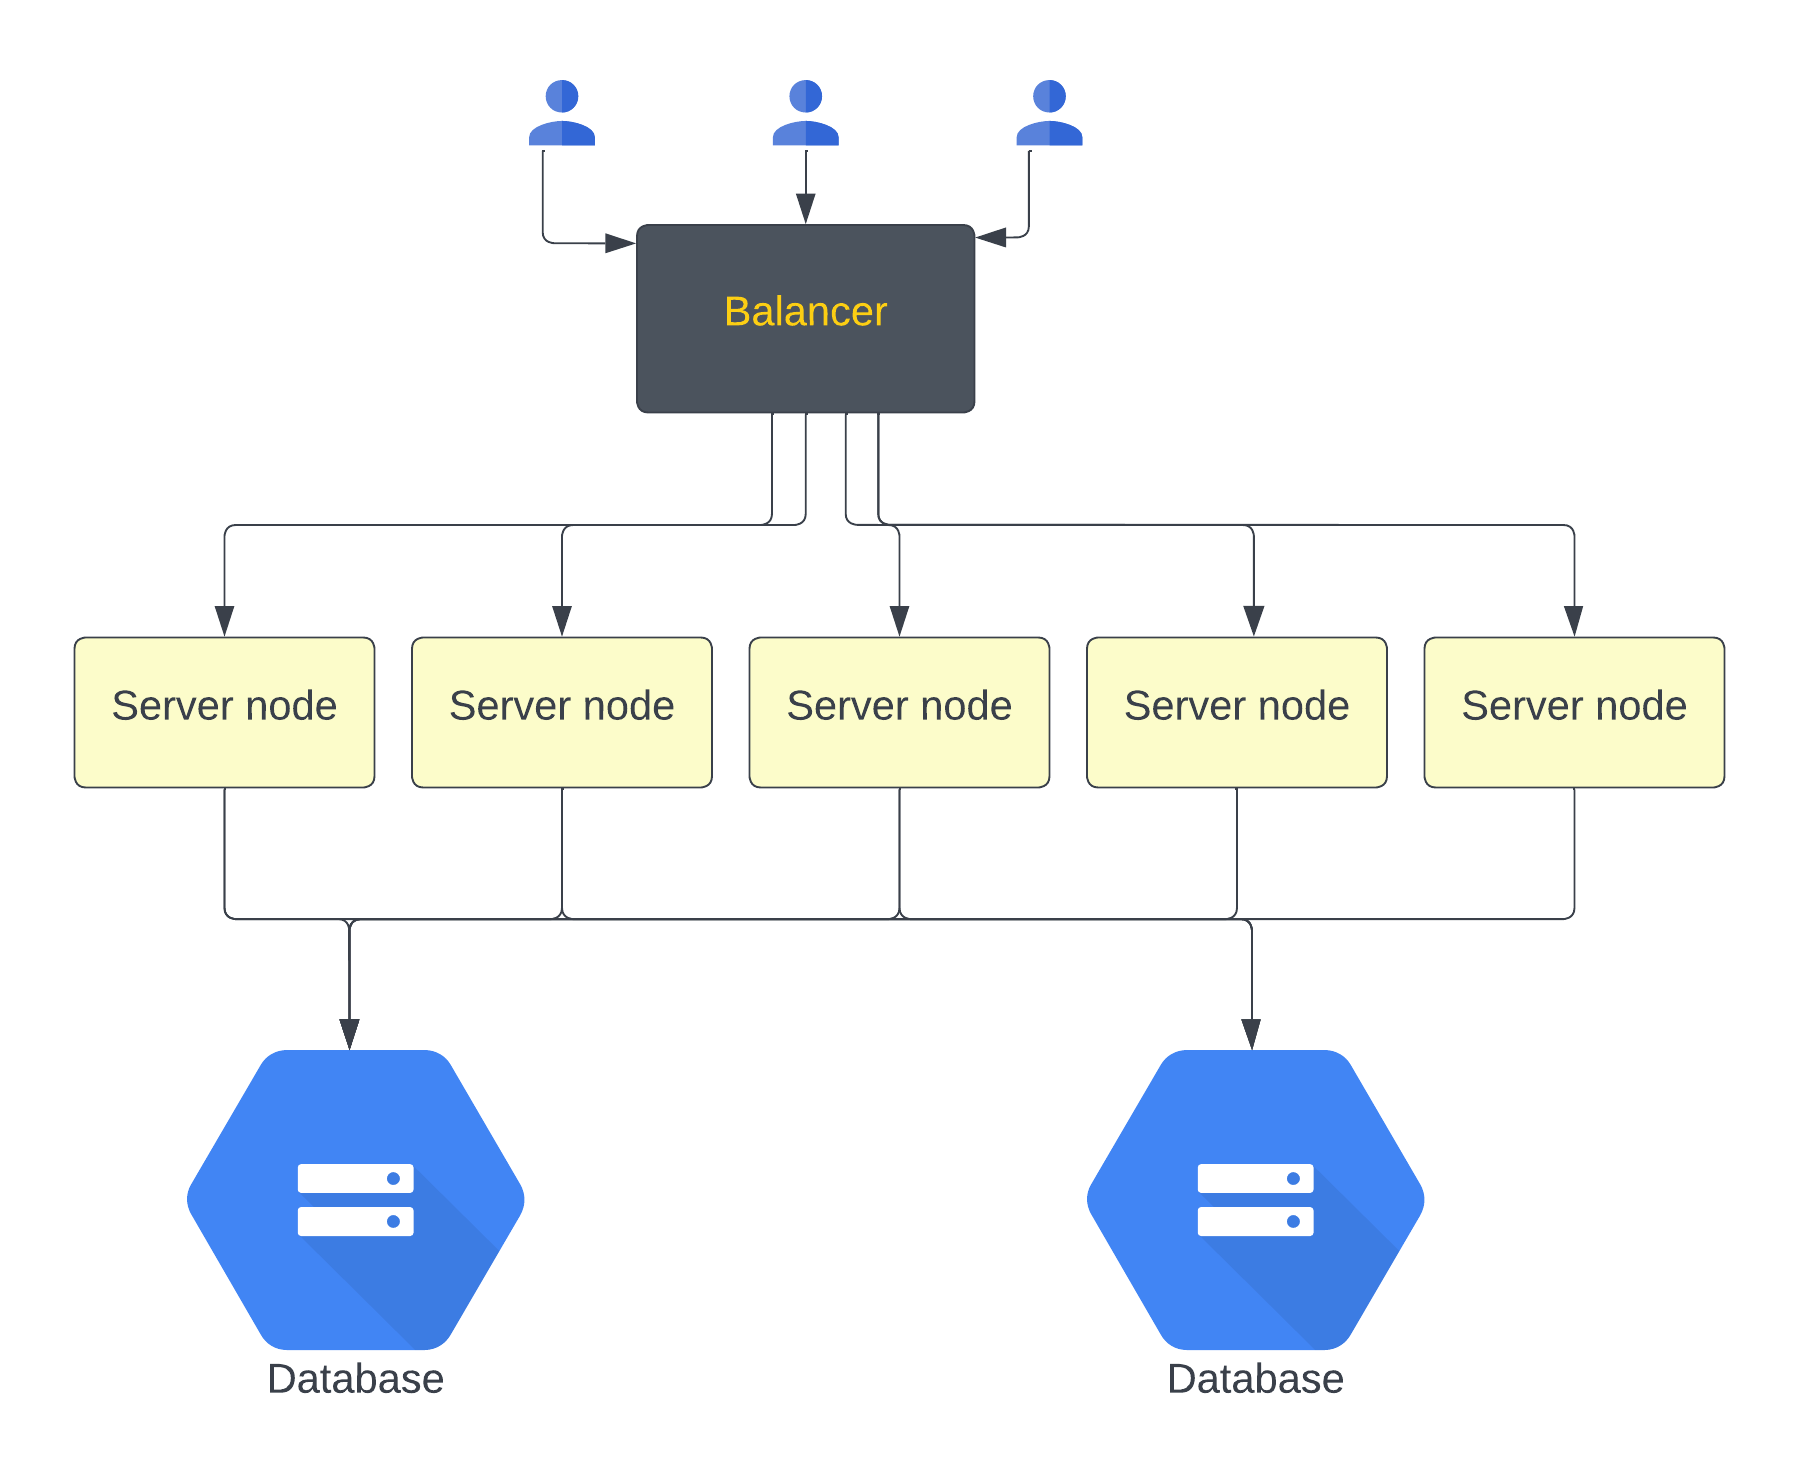
\includegraphics[width=9cm]{images/dist.png}
\end{center}
\end{frame}


\begin{frame}
\frametitle{Требования:}
\begin{itemize}
\item Быстро принимать решение по запросу, отстуствие сетевых блокировок
\item Целостность данных при потере 1 сервера (особый случай обновления)
\item Возможность настройки лимитов и параметров без перезапуска
\end{itemize}
\end{frame}


\begin{frame}
\frametitle{Точность за счёт распределенных хранилищ}
\begin{itemize}
\item Предоставляют доступ к общему состоянию (например реализуя распределенный HashMap)
\item Множество решений, заявляющих высокую производительность: Redis, Ignite, Hazelcast, Infinispan...
\item Для проекта выбран Apache Ignite, оставлена возможность легко перейти на другое решение.
\end{itemize}
\end{frame}

\begin{frame}
\frametitle{Алгоритм и оптимизация скорости.}
\begin{center}
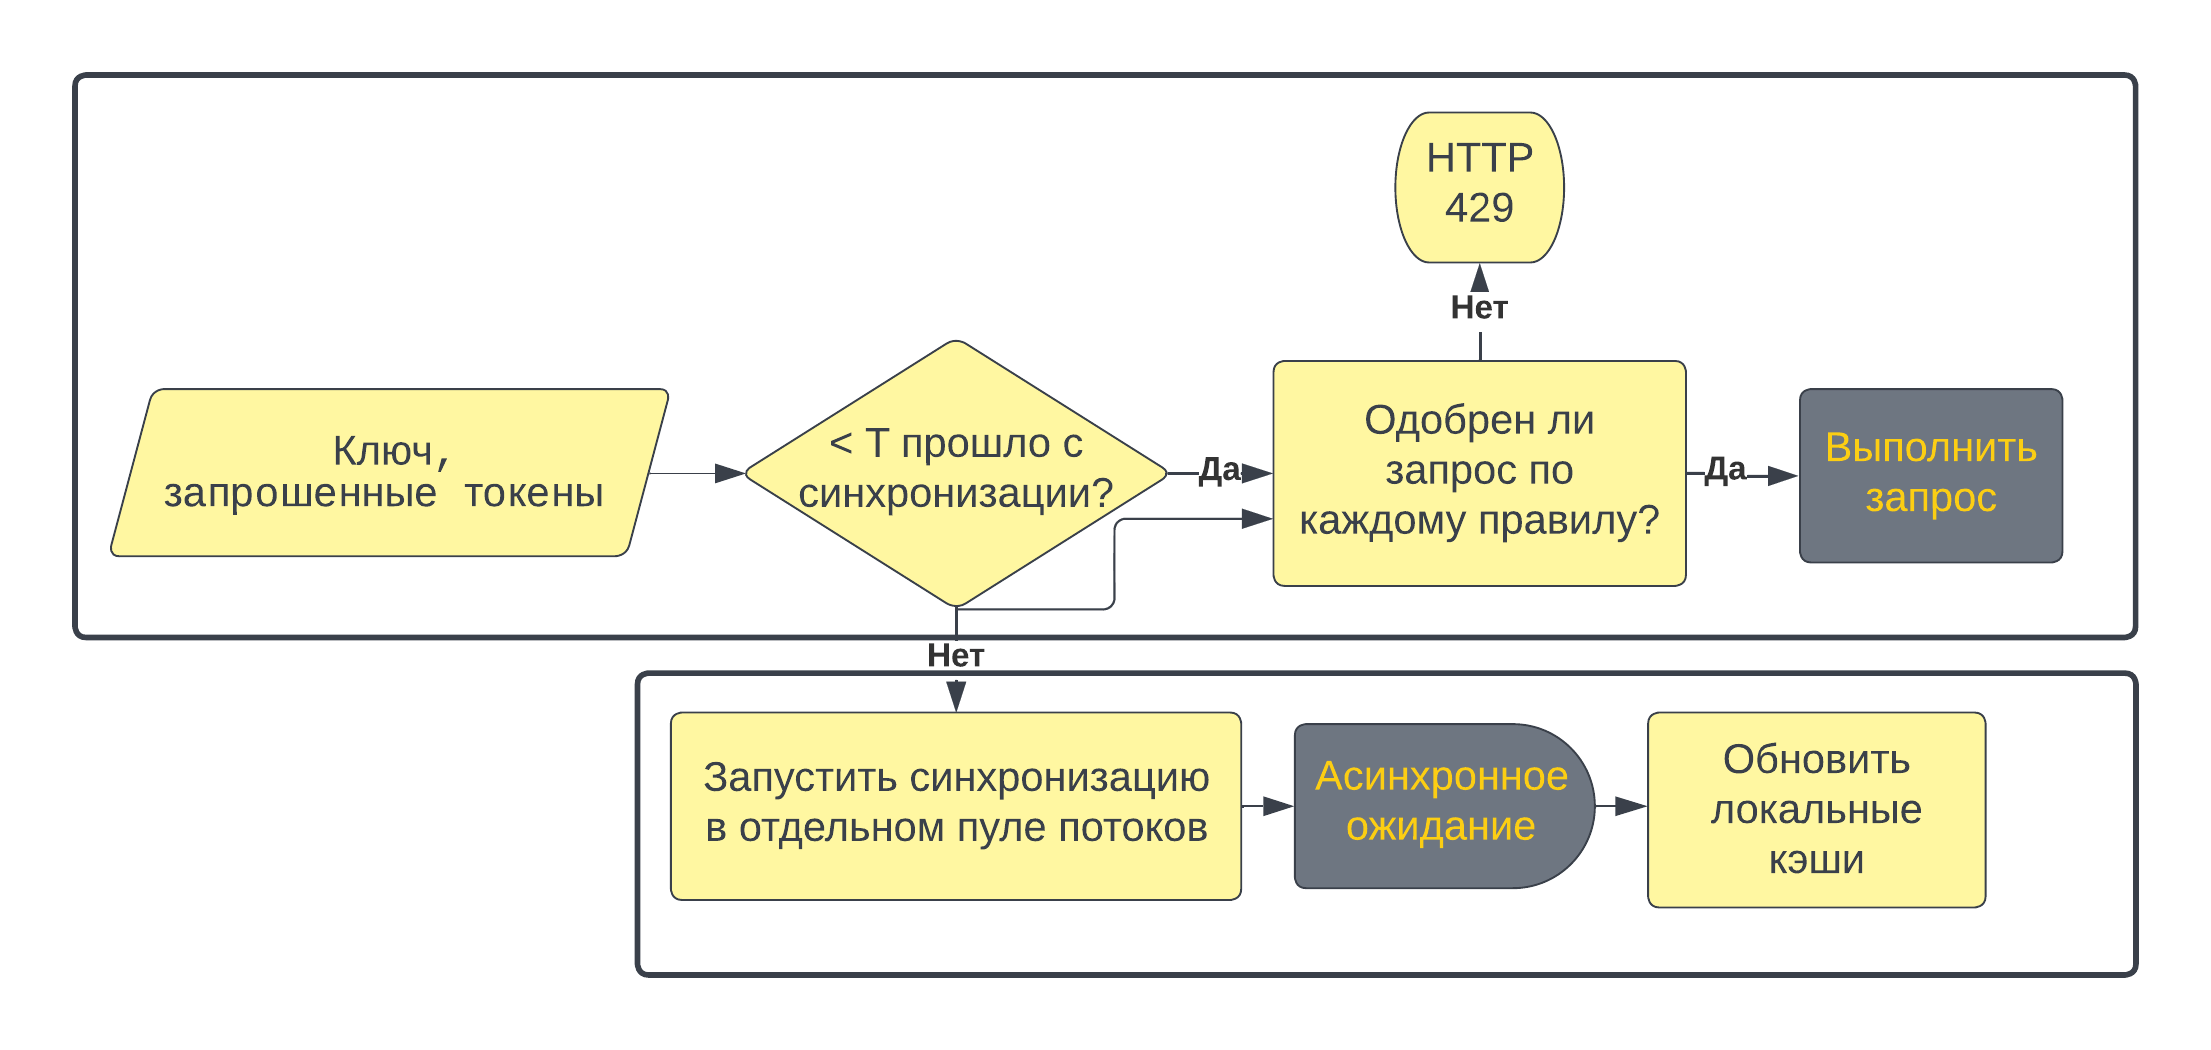
\includegraphics[width=12cm]{images/algoRu.png}
\end{center}
\end{frame}

\begin{frame}
\frametitle{Тесты. CPU}
\begin{center}
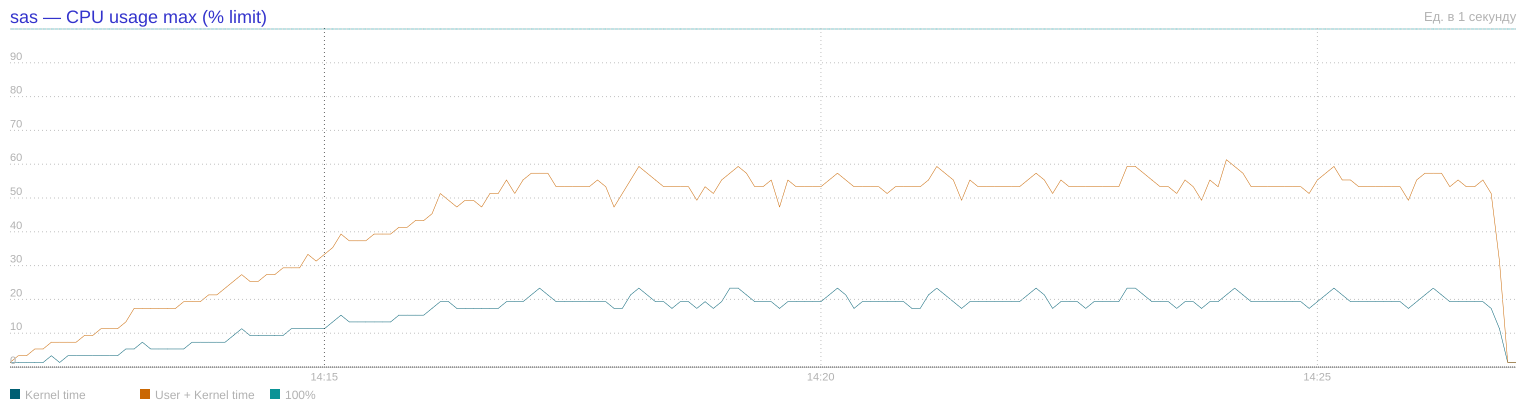
\includegraphics[width=12cm]{images/cpuOff.png}


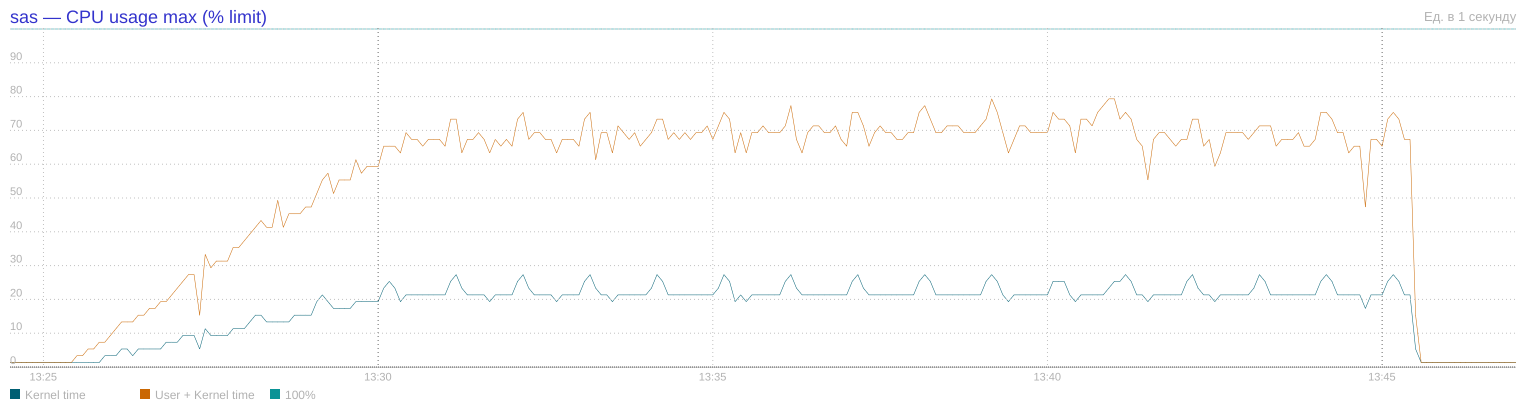
\includegraphics[width=12cm]{images/cpuOn.png}
\end{center}
\end{frame}


\begin{frame}
\frametitle{Тесты. Сеть}
\begin{center}
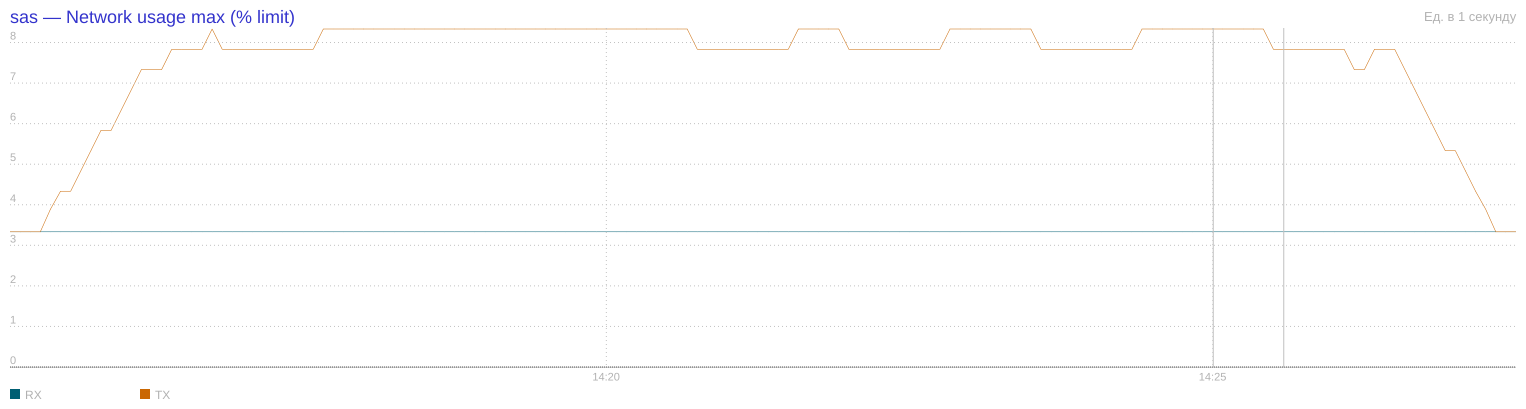
\includegraphics[width=12cm]{images/netOff.png}

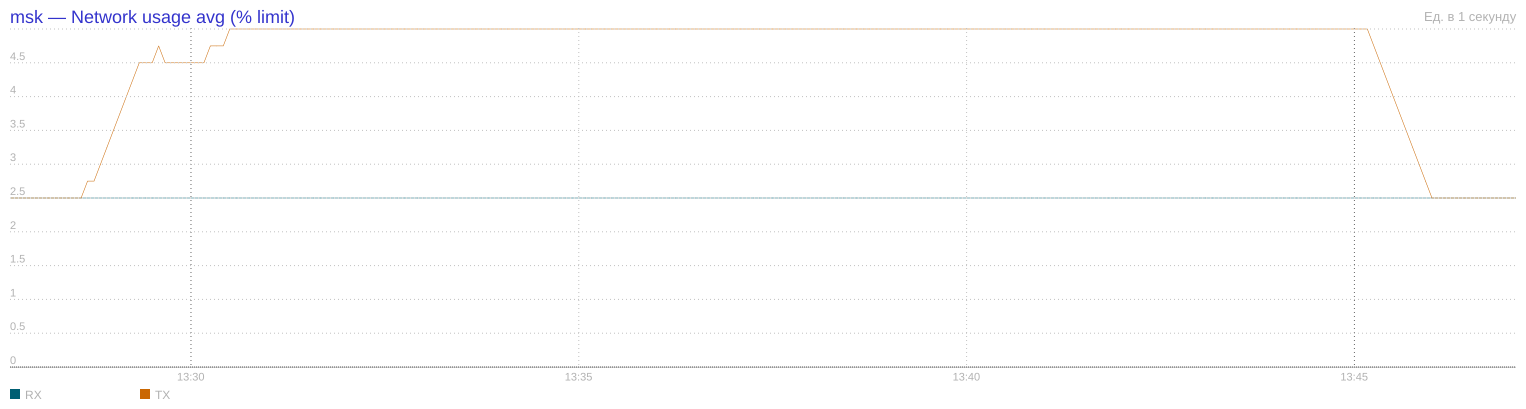
\includegraphics[width=12cm]{images/netOn.png}
\end{center}
\end{frame}

\begin{frame}
\frametitle{Стресс тесты корректности}
\begin{center}
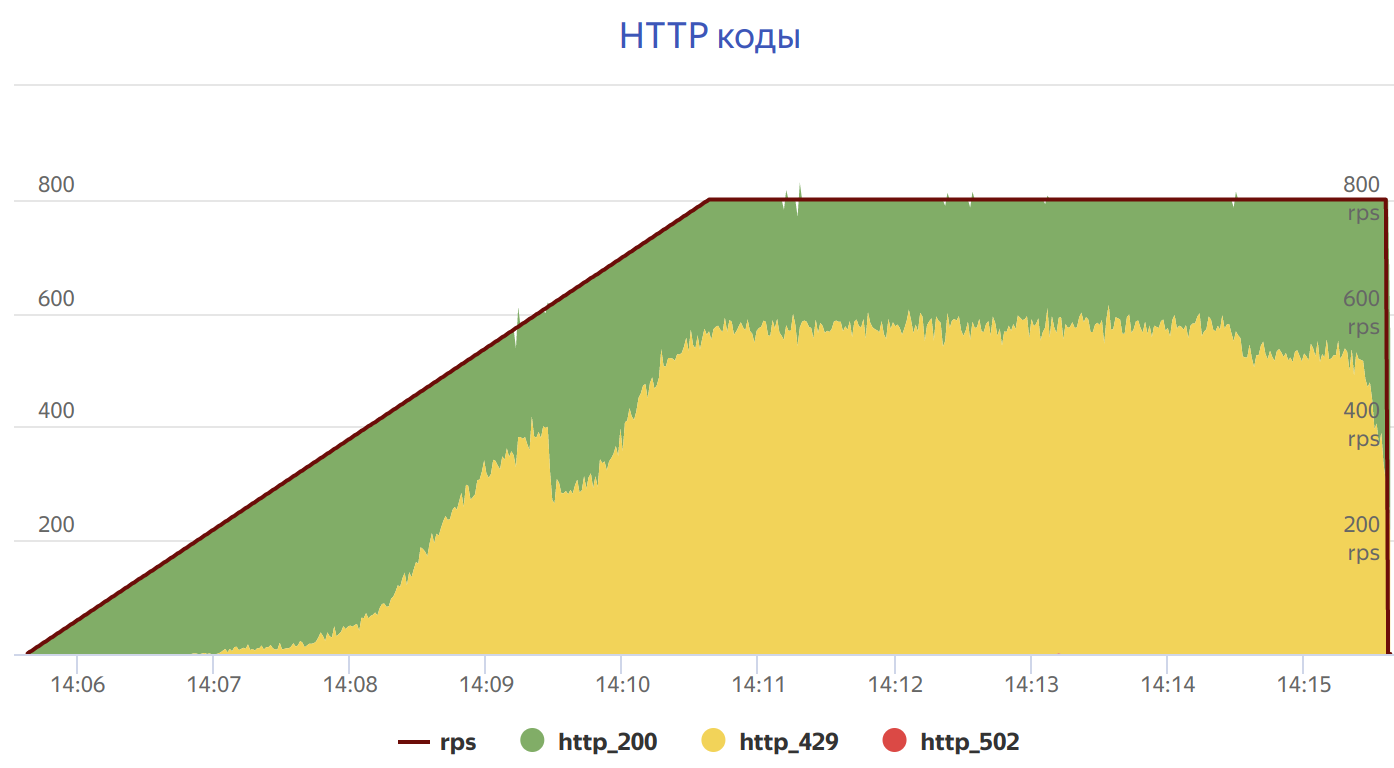
\includegraphics[width=12cm]{images/stress.png}
\end{center}
\end{frame}

\begin{frame}
\frametitle{Основные трудности}
\begin{itemize}
\item Распределенное развертывание не быстрое, прототипирование занимало много времени.
\item В выбранной библиотеке для лимитирование не было важной для проекта функциональности.
\item Не всегда доступны мощности для проведения нагрузочных тестов.
\end{itemize}

\end{frame}

\begin{frame}
\frametitle{Результаты}

\begin{enumerate}
  \item Разработан и протестирован готовый к использованию в Трекере инструмент.
  \item Предоставлен отчёт для команды, содержащий обоснование принятых решений, рекомендации по настройке и работе, а также результаты тестов и их интерпретацию.
  \item Измененная копия отчёта в свободном доступе.
\end{enumerate}

\end{frame}

\begin{frame}
  \frametitle{Ссылки}
  \begin{center}
    Автор: Никита Митцев, muldrik@yandex.ru \\
  \end{center}
  \qrcode[height=45mm]{https://docs.google.com/document/d/1PA6zSGjfig8ZfJeAFRtxucn92N-YWwWgQRYRTN1rkM8/edit?usp=sharing} \hfill
  \qrcode[height=45mm]{https://github.com/muldrik/ratelimiter-presentation/blob/main/slides/slides.pdf}\\
{\small
  \textit{Итоговый отчёт}\hfill
  \textit{Эта презентация}
  % \textit{Итоговый документ (позже переедет в репозиторий выше):} \href{https://docs.google.com/document/d/1XxfN0Q7YrjKV4CA-kIeU_xgnu1CKIoWbNGlGvHUgF9E/edit?usp=sharing}{https://docs.google.com/document/d/1XxfN0Q7YrjKV4CA-kIeU_xgnu1CKIoWbNGlGvHUgF9E/edit?usp=sharing}
%   \textit{Репозиторий с кодом для сбора статистики:} \href{https://github.com/muldrik/projector-server}{https://github.com/muldrik/projector-server}\\
%   \textit{Репозиторий с кодом для генерации отчётов и графиков:} \href{https://github.com/muldrik/projector-report-generator}{https://github.com/muldrik/projector-report-generator}
}
\end{frame}



\end{document}
